\documentclass{article}
\setlength{\headheight}{23pt}
\usepackage[utf8]{inputenc}
\usepackage[a4paper, margin=1in]{geometry}
\usepackage{multicol}
\usepackage{amsmath}
\usepackage{fancyhdr}
\usepackage{float}
\usepackage{graphicx, subfigure}
\usepackage{titlesec}
\usepackage{multirow}

\usepackage[dvipsnames]{xcolor}
\usepackage{soul}
\newcommand{\ctext}[3][RGB]{%
  \begingroup
  \definecolor{hlcolor}{#1}{#2}\sethlcolor{hlcolor}%
  \hl{#3}%
  \endgroup
}

\titleformat{\section}[frame]
{\normalfont} {} {2pt} {\Large\bfseries\filright\thesection.\quad}

\title{EECS 470 Cheat Sheet}
\author{khtaur }
\date{Janurary 2021}

\pagestyle{fancy}
\fancyhf{}
\fancyhead[R,RO]{Ke-Haur Taur\\khtaur@umich.edu}
\fancyhead[L,LO]{University of Michigan\\EECS 470 W21}
\fancyhead[C]{Computer Architecture\\Concept Cheat Sheet}
\fancyfoot[C]{\thepage}
\fancyfoot[L]{Ke-Haur Taur}
\renewcommand{\headrulewidth}{1pt}
\renewcommand{\footrulewidth}{1pt}

\begin{document}

\begin{multicols*}{2}

\section{Roadmap}
\begin{figure}[H]
  \centering
    {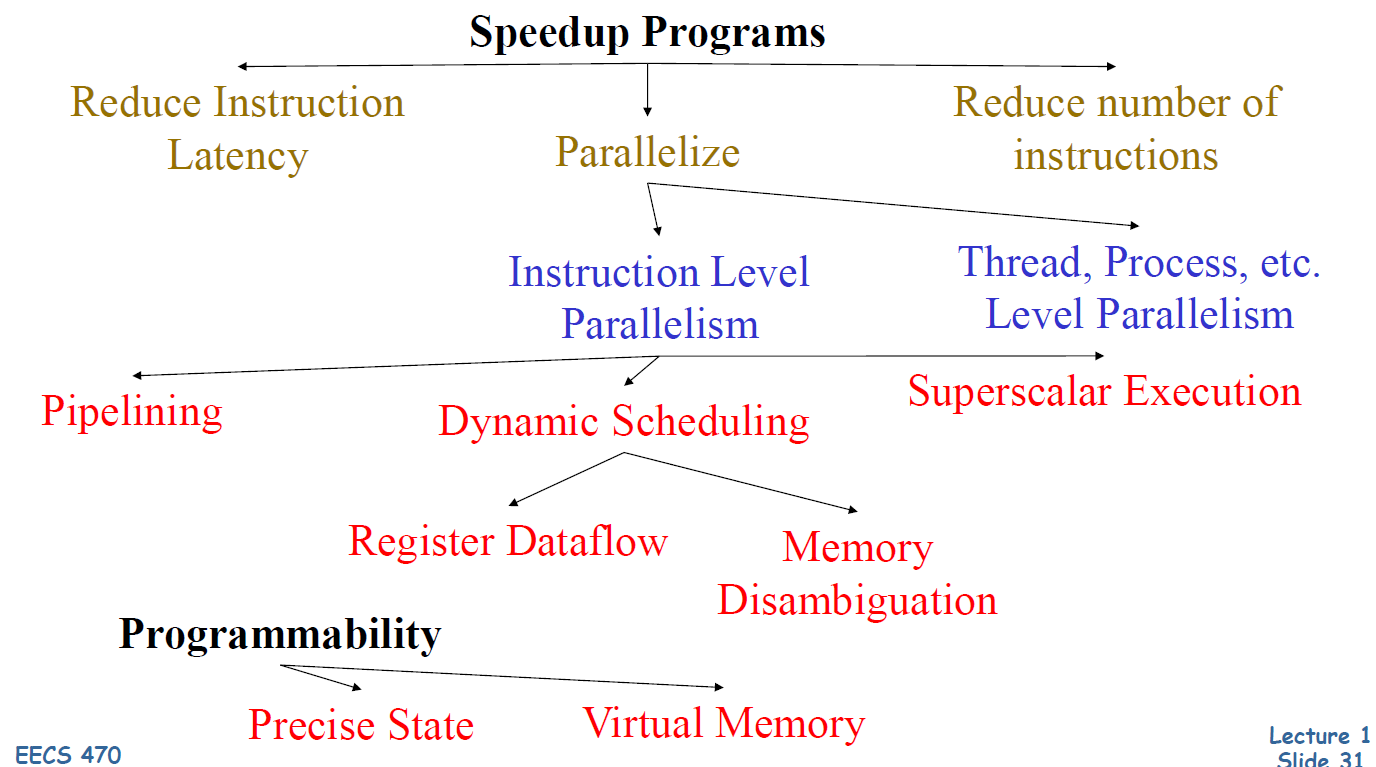
\includegraphics[width=.4\textwidth]{1.png}}
  \caption{EECS 470 Roadmap}
\end{figure}

\section{Performance Metrics}
\subsection*{Amdahl's Law}
Define Speedup $S = \frac{t_{\text{With}}}{t_{\text{Without}}}$ 
\medskip\par\noindent
Speeds up fraction $f$ of task by factor of $S$ \\
$\rightarrow S = \frac{1}{(1-f)+\frac{f}{S}}$
\medskip\par\noindent
Consider how size of $f$ affects speedup?

\subsection*{Averaging Methods}
Latency($A+B$) = Latency($A$) + Latency($B$)\\
Thru($A+B$) != Thru($A$) + Thru($B$)
\medskip\par\noindent
Should be \textit{Harmonic}: $\frac{1}{\frac{1}{\text{Thru}_A} + \frac{1}{\text{Thru}_B}}$ since Ratios cannot be added directly! Applies to other units inversely proportional to time.
\medskip\par\noindent
Other averaging methods: \textit{geometric} (for unitless quantities)

\subsection*{Iron Law}
Performance $P$ = (code size) $\cdot$ (CPI) $\cdot$ (Cycle time) \\
Clock Frequency = Cycles per second

\section{ISA and Power}
\subsection*{RISC and CISC}
ISA is the contract between HW and SW \\
RISC: \\
(1) Many single-cycle instructions $\rightarrow$ higher CPI \\
(2) Larger code size \\
(3) Allows faster clock

\subsection*{Capacitive Power Model}
Power $\approx \frac{1}{2}CV^2f$ \\
Frequency and Voltage scales together \\
$\rightarrow CV^2f = CV^3$ \\
80\% Power = Voltage drop 7\% or $(.93^3)$

\subsection*{Voltage Scaling}
Reduce to 80\% Performance $\rightarrow$ used only 50\% Power! ($.8^3 \approx 0.5$) \\
If fully-parallel $\rightarrow$ 160\% Performance with the same energy budget! 

\section{Cache Architecture}
\begin{figure}[H]
  \vspace*{-1cm}
  \centering{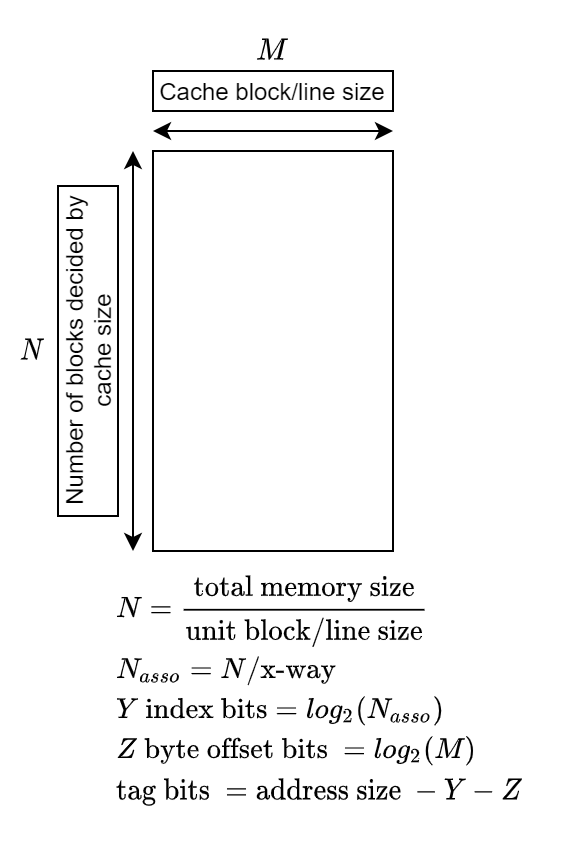
\includegraphics[width=.4\textwidth]{cache.png}}
  \vspace*{-.5cm}
  \caption{Cache Structure}
\end{figure}

Why need caches in the first place? To utilize locality. \textbf{Locality is expressed with different lower bits} and the same higher bits.

\begin{figure}[H]
  \centering{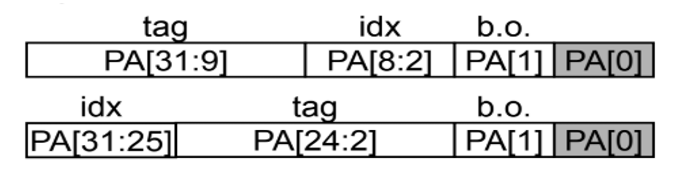
\includegraphics[width=.4\textwidth]{11.png}}
  \caption{Get which part of PA as index to cache?}
\end{figure}

\subsection*{N-way associativity (N=2)}
\begin{figure}[H]
  \centering{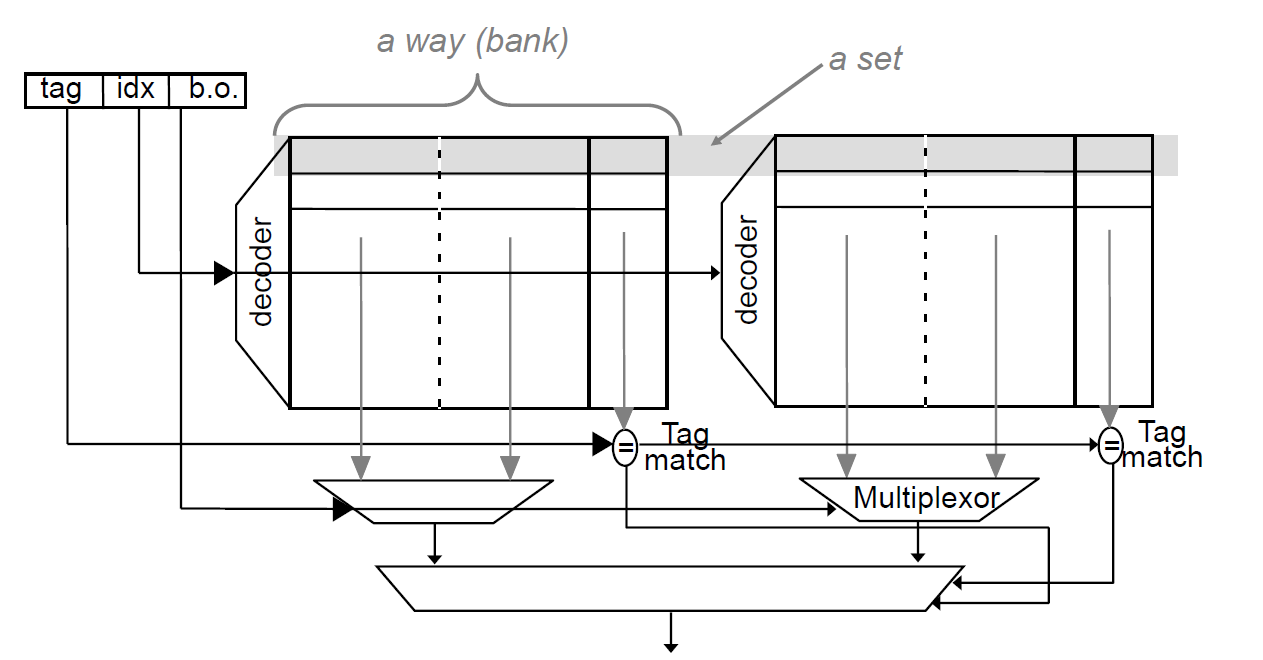
\includegraphics[width=.45\textwidth]{15.png}}
  \caption{Cache Structure Hardware}
\end{figure}

\subsection*{Cache Write Policies}
On \textbf{W Hits}: \textbf{Write-through} writes upon block update while \textbf{Write-back} updates upon block eviction. \\
On \textbf{W Misses}: \textbf{Write-Allocate} brings whole block frame to utilize locality while \textbf{no-write-allocate} only allocates for real misses.

\subsection*{Regular Associativity vs Skewed}
Skewed associativity uses \textbf{different hash functions} to index \textbf{each} way to \textbf{reduce conflict misses}. A hash XORs different sets (e.g., [21:15] and [14:8]) of bits of given address instead of using designated tag bits (regular).

\begin{figure}[H]
  \centering{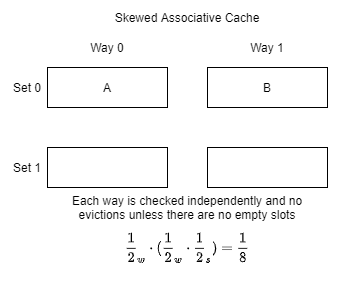
\includegraphics[width=.4\textwidth]{12.png}}
\end{figure}

\begin{figure}[H]
  \centering{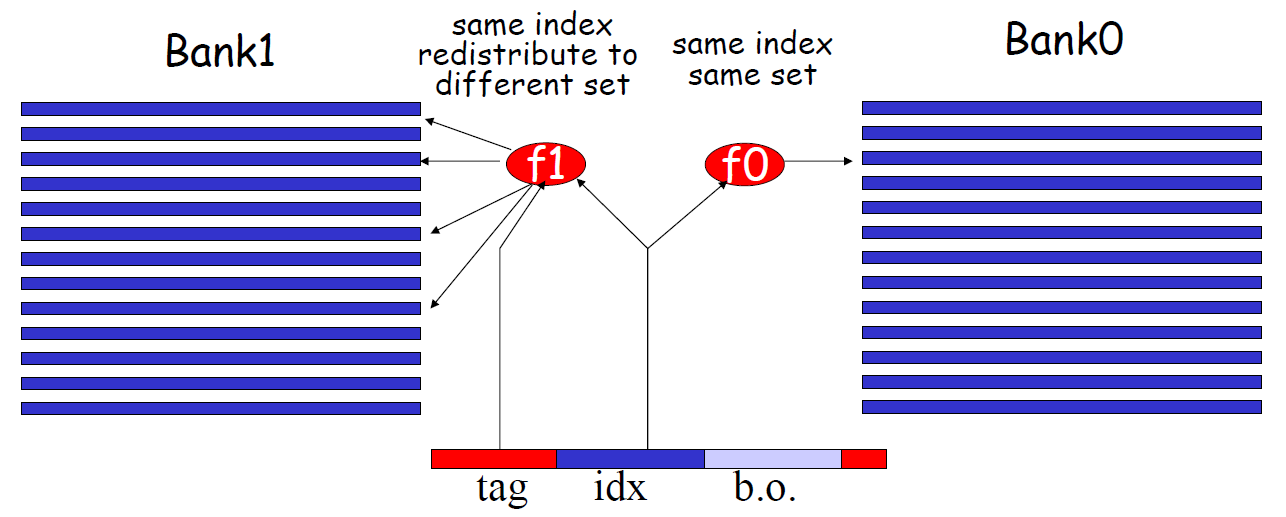
\includegraphics[width=.45\textwidth]{13.png}}
  \caption{Skewed Associative Caches}
\end{figure}

\subsection*{Cache Average Access Time}
Multi-level cache access times can be formulated recursively. (Assuming only L1 and L2 and are accessed in series)
\begin{alignat*}{3}
    &t_{\text{L1 Avg}} &&= t_{\text{L1 Hit}} &&+ \text{(L1 Miss Ratio)} \cdot t_{\text{L2 Avg}} \\
    &t_{\text{L2 Avg}} &&= t_{\text{L2 Hit}} &&+ \text{(L2 Miss Ratio)} \cdot t_{\text{Memory}}
\end{alignat*}
Global Miss ratio: L2 Misses/ L1 accesses \\
Local Miss ratio: L2 Misses/ L1 misses (Bad if L1 high hit rate)

\subsection*{Large Blocks and sub-blocks}
Critical word first transfers requested word-size to processor before rest of cache block.
\medskip\par\noindent
Implemented with a sub-blocked cache where each sub-block has its own valid bit. Sub-blocked caches still have smaller tag arrays (less sets) while have less transfer overhead (Critical word first).

\subsection*{Cache Inclusion Violation}
If L2 is not guaranteed to be the super-set of L1, than when L1 evicts a block to L2, L2 may run into a store miss before accepting the evicted block. (Stalls L1 eviction which is very slow)\\
Instead, flush L1 block (back-invalidation) if it does not exist in L2.

\begin{figure}[H]
  \centering{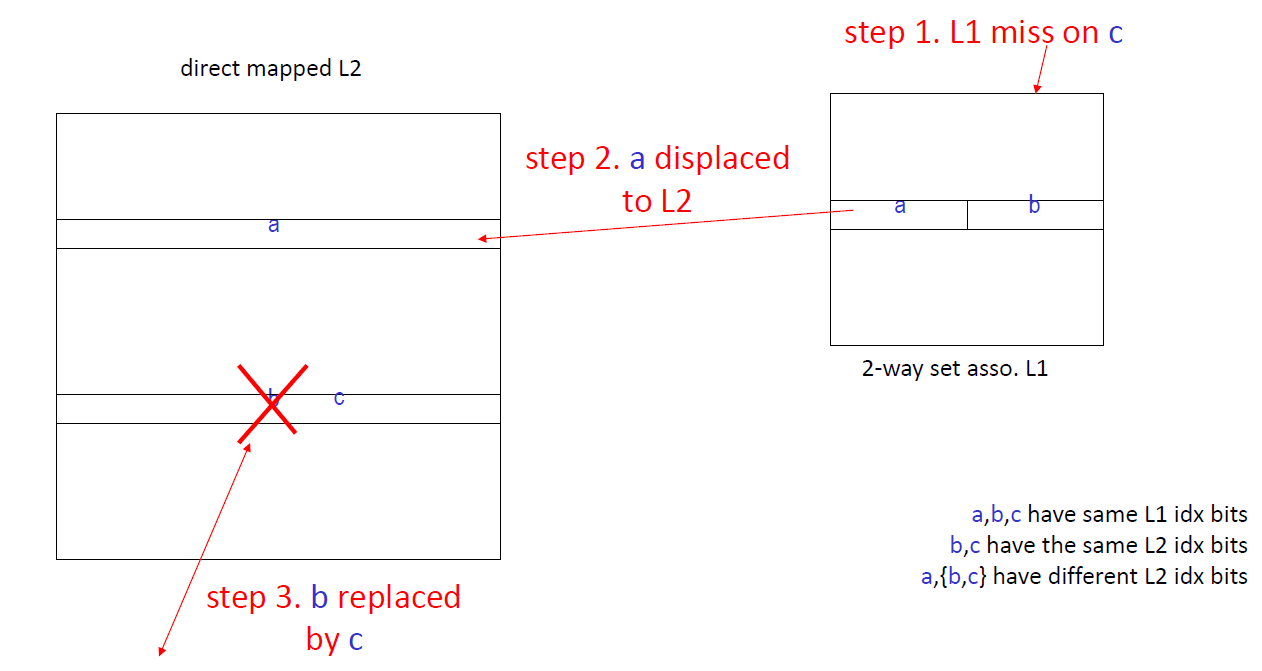
\includegraphics[width=.45\textwidth]{16.png}}
  \caption{Possible Inclusion Violation}
\end{figure}

\noindent
The figure assumes that b is more recently accessed in L1.

\subsection*{Non-blocking Caches}
Miss status holding registers (MSHR) keeps track of load/store misses and handle the requests in order (if the main memory is pipelined). Possible optimizations include \textbf{load coalescing} when no stores are between in the two loads.

\section{The Execution Core}
3 Ways to speed up a process:\\
Reduce tasks/Decrease latency/Parallelize
\medskip\par\noindent
Single-Cycle $\rightarrow$ Multi-Cycle $\rightarrow$ Parallel-Multi-Cycle (Superscalar) $\rightarrow$ Pipelining

\subsection*{Pipeline Hazards}
The longer the pipeline is (more stages), the longer the chain of dependencies is; hence more chances to stall.\\
\medskip\par\noindent
Data Dependencies: \textbf{RAW} \\
Need to consider RAW hazards, next instruction can decode when current instruction is writing back. Can either \textbf{Avoid} (Compiler insert NOPs), \textbf{Stall} (Pass NOP to EX) or \textbf{Forward} data.
\medskip\par\noindent
Control Dependencies: \\
Can either \textbf{Detect and Stall} (Hold next instruction in Fetch) or \textbf{Speculate and Squash} (Hazard found at EX, pass NOP to previous stages and target to Fetch).

\subsection*{Scoreboarding}
Why? (1) IPC bottleneck, (2) Long latency and (3) Too much stalls. \medskip\par\noindent
New Scoreboard Pipeline: F, D, S, X, W \\
\smallskip\hrule\smallskip\noindent
{[W]}: Check for WAR Hazards (un-flagged register entry in FU status)? Wait till hazard is resolved; Otherwise, write to dest register and free entry in status table. \textbf{Why WAR?} An younger inst can potentially overwrite the dependency of an un-issued older inst. \\
\smallskip\hrule\smallskip\noindent
{[X]}: Execute and notify scoreboard when done \\
\smallskip\hrule\smallskip\noindent
{[S]}: Check for RAW Hazards? Wait till hazard is resolved and pending register status is cleared; Otherwise, Read register values \\
\smallskip\hrule\smallskip\noindent
{[D]}: Check for WAW (non-empty Register-status table entry) and FU Structural hazards? Stall if hazards are present; Otherwise, allocate entry in status table. \textbf{Why WAW?} An younger inst can overwrite a register that an older inst is attempting to write and insts in between can read the wrong value.\\
\smallskip\hrule\smallskip\noindent
{[F]}: Same instruction fetch in MIPS 5 stage pipeline

\begin{figure}[H]
  \centering
    {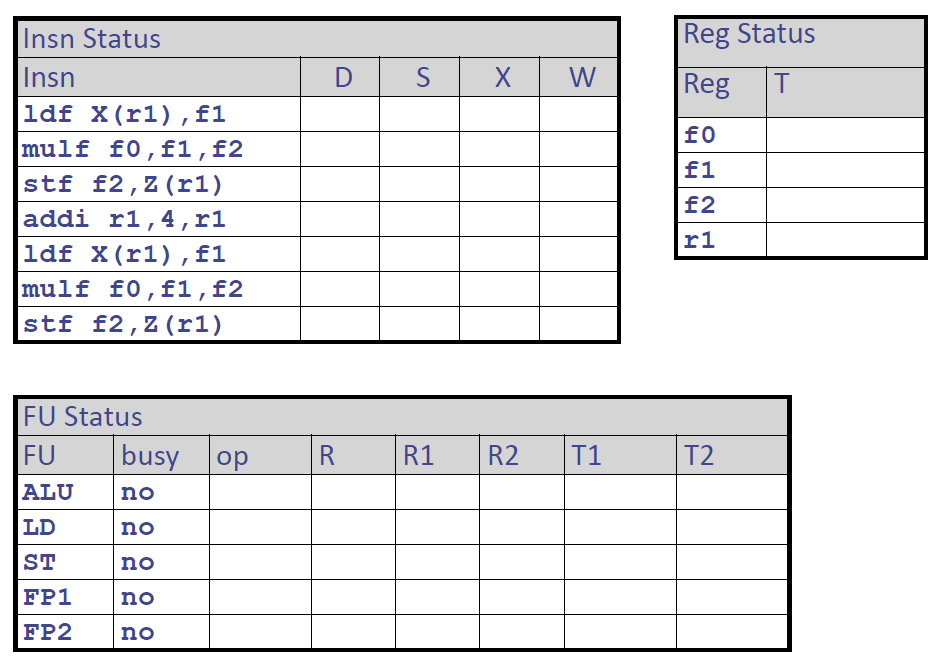
\includegraphics[width=.49\textwidth]{2.png}}
  \caption{Scoreboard Data Structure}
\end{figure}

\medskip\par\noindent
\textbf{What's good of scoreboard:} \\
(1) Cheap Hardware \\
\medskip\par\noindent
\textbf{What's less good of scoreboard?} \\
(1) RAW inst take a long time to issue and delays WARs \\
(2) Can be fixed with register renaming


\subsection*{Tomasulo}
Why? Register renaming in hardware! $\rightarrow$ Meaning that process can have \textbf{multiple active versions} of same name! Combines Register Renaming and Dynamic Scheduling. Values of architectural registers are recorded in every entry of the RS.
\medskip\par\noindent

\medskip\par\noindent
\smallskip\hrule\smallskip\noindent
{[W]}: Clear register matching RS entry in map table and free corresponding RS entry. CDB broadcasts information carried by the register to those who need it. \\
\smallskip\hrule\smallskip\noindent
{[X]}: Executes instruction with data passed from RS\\
\smallskip\hrule\smallskip\noindent
{[S]}: Check for RAW Hazards? Wait till hazard is resolved and CDB passes needed values; Otherwise, proceed with values in RS. \\
\smallskip\hrule\smallskip\noindent
{[D]}: Check for Structural hazards? Stall if hazards are present; Otherwise, allocate entry in RS and copy architectural register value from map table if available. Then record the renamed destination register in the map table. \\
\smallskip\hrule\smallskip\noindent
{[F]}: Same instruction fetch in MIPS 5 stage pipeline

\begin{figure}[H]
  \centering
    {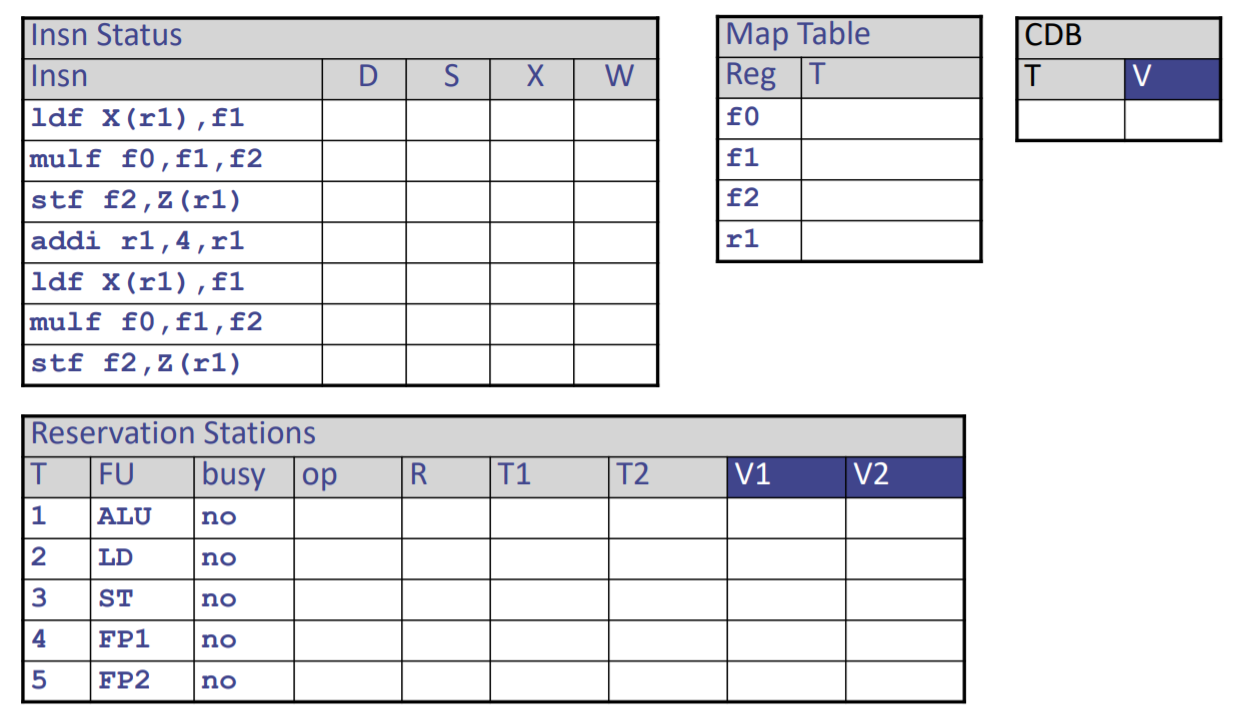
\includegraphics[width=.49\textwidth]{3.png}}
  \caption{Tomasulo Data Structure}
\end{figure}

\subsection*{Scoreboard and Tomasulo summary}
\textbf{Dynamic Scheduling:} \\
Higher overall FU utilization
\medskip\par\noindent
\textbf{Instruction Buffer:} \\
Split Decode stage into Issue and Dispatch. Instructions dispatch in-order while issue is out-of-order.
\medskip\par\noindent
\textbf{Register Renaming:} \\
Observation is that WAR/WAW hazards can be avoided if there are unlimited registers. Can be thought as a dependency chain: destination registers are renamed upon encountering a write to a architectural register. Younger instructions can safely proceed to write to their own renamed copies. Instructions in between an older and younger counterpart would receive the correct renamed-write from the CDB.
\medskip\par\noindent
\textbf{Algorithms:} \\
\textbf{Scoreboard} records FU unit writing to the architectural register in the Map Table instead of renaming which is employed in \textbf{Tomasulo} (rename using RS entry). Renaming creates a dependency timeline so all Write-After hazards are eliminated.

\subsection*{OoO Caveats}
\subsubsection*{OoO hard bypassing}
Younger instructions have to "arrive early" to receive the forwarded data; hence pipeline has to be modified in terms of architecture.

\subsubsection*{OoO Interrupts/Exceptions}
Need to include semantics: All insts \textbf{before} interrupt should be complete and All insts \textbf{after} interrupt should look as if never started (abort)
\medskip\par\noindent
Hard because OoO has to undo post-interrupt writebacks; Hence the need of implementing precise state in OoO.

\subsection*{OoO Precise State}
OoO Writeback combines 2 functions: (1) Forward values to younger instructions (2) Overwrite values in register file. (2) requires in-order sequence.
\medskip\par\noindent
Similar to splitting decode, split writeback into (1) \textbf{complete} and (2) \textbf{retire}. Instructions \textbf{complete} out-of-order and \textbf{retire} in-order.

\section{P6 Case Study (Lec 7)}

\begin{figure}[H]
  \centering
    {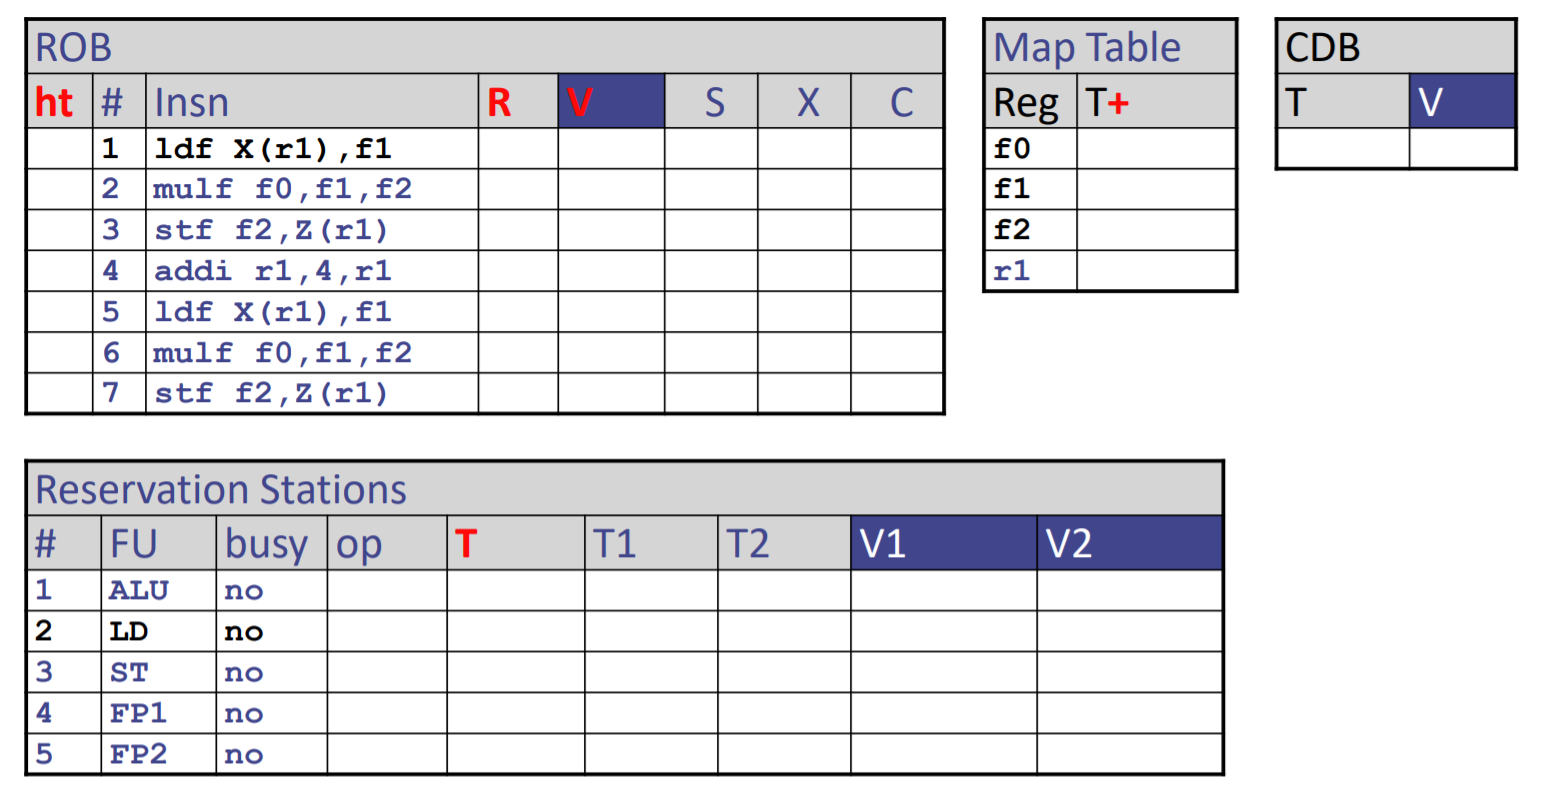
\includegraphics[width=.49\textwidth]{4.png}}
  \caption{P6 Data Structure}
\end{figure}

\subsection*{Stepping through the P6 architecture}
[R]: See if Retire is eligible (if the head pointer is not here yet, stall). (1) Write Value to dest ARF and (2) Advance head pointer and clear CDB.
\smallskip\hrule\smallskip\noindent
{[C]}: See if eligible to (1) broadcast to CDB and (2) CAM Map Table $+$ tag and set values for corresponding ROB\# tags in RS.
\smallskip\hrule\smallskip\noindent
{[X]}: See if eligible to free RS entry \\ 
(Inst freed from RS when reach X stage). \smallskip\hrule\smallskip\noindent
{[S]}: See if eligible to get tag values from CDB or Map Table entry that has ready bit.
\smallskip\hrule\smallskip\noindent
{[D]}: See if RS is eligible to allocate a FU entry and fill corresponding tags (Dest/T1/T2/V1/V2). Rename destination register with ROB entry

\subsection*{P6 architecture Performance}
Added ROB is not a performance addition, but handles exceptions unlike Tomasulo which doesn't. Performance more or same as Tomasulo if ROB size is chosen wisely (at least Width $\cdot$ Num\textsubscript{stages D-R})

\section{R10K Case Study (Lec 9)}

\begin{figure}[H]
  \centering
    {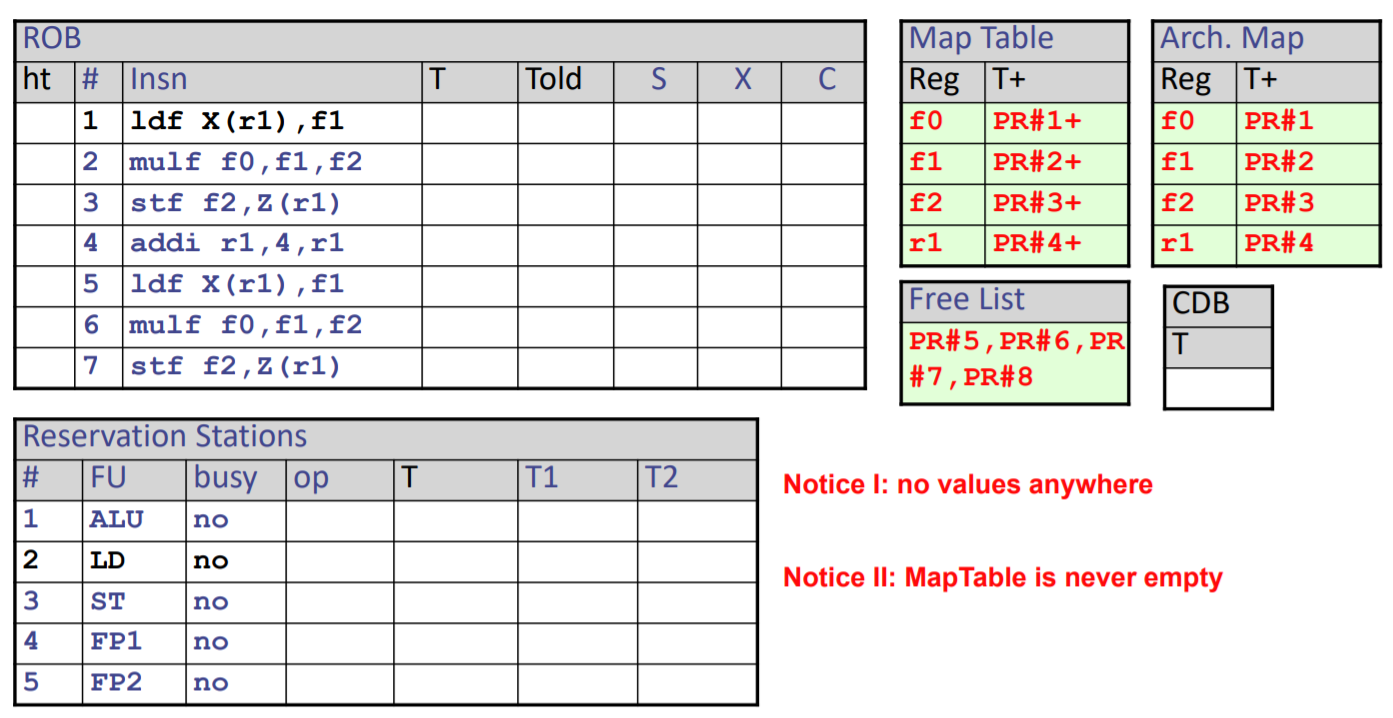
\includegraphics[width=.49\textwidth]{5.png}}
  \caption{R10K Data Structure}
\end{figure}

\subsection*{Stepping through R10K}
[R]: If retire is eligible, (1) return T\textsubscript{old} to Free list (2) update T in Arch-Map and (3) advance head pointer and clear CDB.
\smallskip\hrule\smallskip\noindent
{[C]}: See if Complete is eligible to (1) set T in CDB and (2) CAM Map Table/RS and set corresponding ready bit. If T of current inst $\neq$ T of corresponding ARF in the Map Table, don't set $+$ bit.\\
(Ready bit in Map Table notifies younger insts)
\smallskip\hrule\smallskip\noindent
{[X]}: Free corresponding RS entry. \\ 
(Inst freed from RS when reach X stage)
\smallskip\hrule\smallskip\noindent
{[S]}: See if Issue is eligible to issue tag when CDB has matching tag or T in Map Table entry has all ready bits set.\\
(Check Dependencies of Inst at S stage)
\smallskip\hrule\smallskip\noindent
{[D]}: See if RS is eligible to (1) allocate a FU entry then fill dest/souce tag values and (2) get T from Free list. Record original tag in Map Table in T\textsubscript{old}.

\subsection*{R10K without Arch-Map}
Maintaining a Arch-Map is expensive. But the architecture still has to guarantee precise state despite the removal of the Arch-Map.
\begin{figure}[H]
  \centering
    {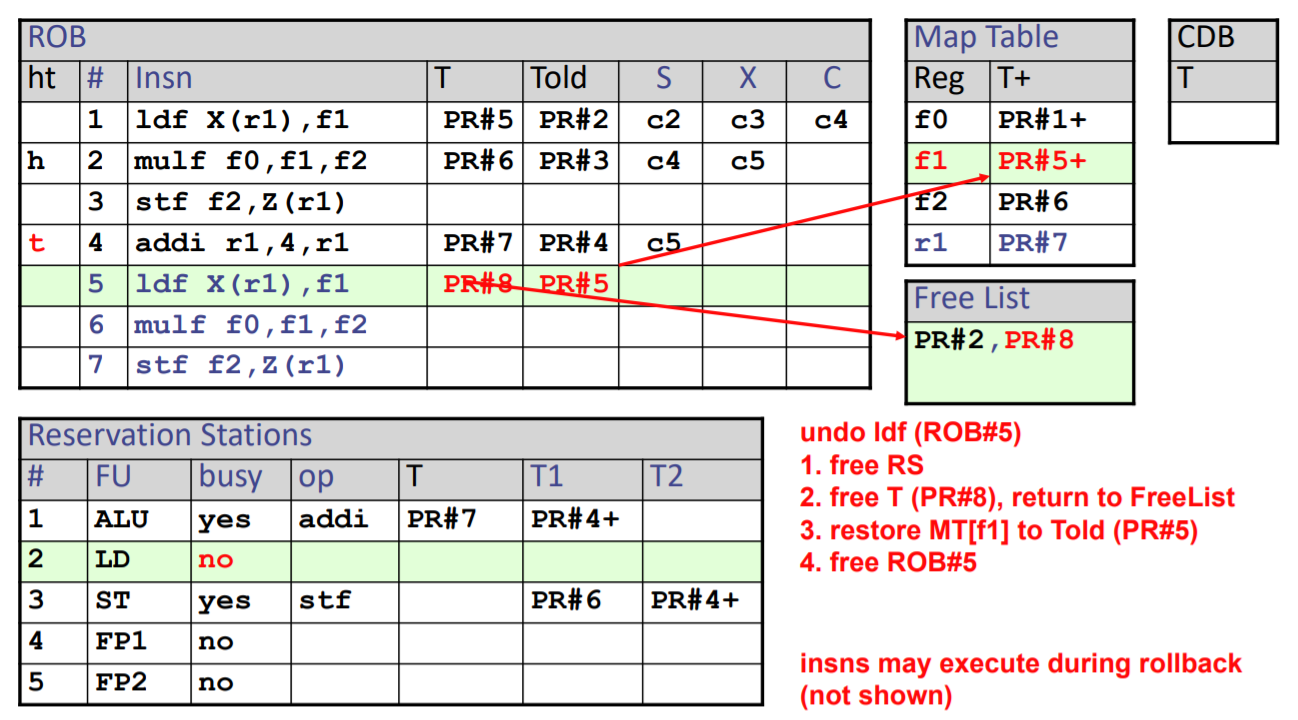
\includegraphics[width=.49\textwidth]{6.png}}
  \caption{R10K without Arch. Map}
\end{figure}

\noindent
As shown in the figure, redo each inst and move the tail pointer up.


\section{R10K V.S. P6}
ARF stands for Architectural RF while PRF stands for Physical RF. P6 has a lot more data movement but has easier precise state recovery.
\begin{figure}[H]
  \centering
    {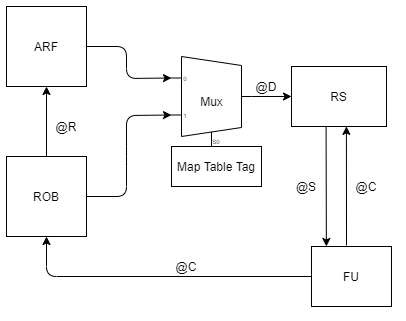
\includegraphics[width=.4\textwidth]{7.png}}
  \caption{P6 Data Movement}
\end{figure}

\begin{figure}[H]
  \centering
    {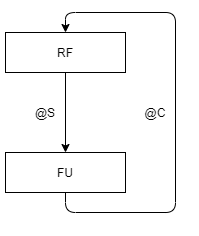
\includegraphics[width=.2\textwidth]{8.png}}
  \caption{R10K Data Movement}
\end{figure}

\section{Memory Disambiguation}
Storing to memory is irrevocable and memory dependencies are not static: addresses need to be calculated first.

\subsection*{Load Handling Strategies}
{[1]}: Allow only one load or store in OoO core. Wait until the previous memory op has finished.
\medskip\hrule\medskip\noindent
{[2]}: Load may only issue when all older memory ops have finished.
\medskip\hrule\medskip\noindent
{[3]}: If alias between a load and an earlier store, forward the value from within the LSQ

\subsection*{OoO Load Execution with the SQ}
{[1]}: Send load address to SQ and compare (CAM) with all store addresses.
\medskip\hrule\medskip\noindent
{[2]}: Select all matching addresses in SQ.
\medskip\hrule\medskip\noindent
{[3]}: If match(s), age logic selects \textbf{youngest store that is older than load (load position input)}
\medskip\hrule\medskip\noindent
{[4]}: If no matches, Load gets value from D\$
\begin{figure}[H]
  \centering
    {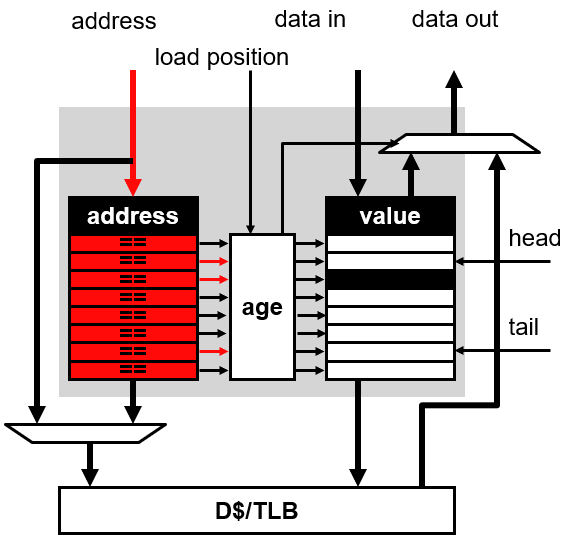
\includegraphics[width=.45\textwidth]{10.png}}
  \caption{Load and SQ}
\end{figure}

\subsection*{Speculative Load with the LQ and SQ}

In this configuration with both SQ/LQ, loads can issue OoO w.r.t. stores. 

\noindent
{[X]}: When loads execute, it CAMs the SQ for forwarding opportunities. When stores exeute, it CAMs the LQ for mis-issued loads that require exception handling.
\medskip\hrule\medskip\noindent
{[D]}: The RS records the SQ/LQ entry of each instruction during dispatch.

\begin{figure*}[ht]
    \centering
    {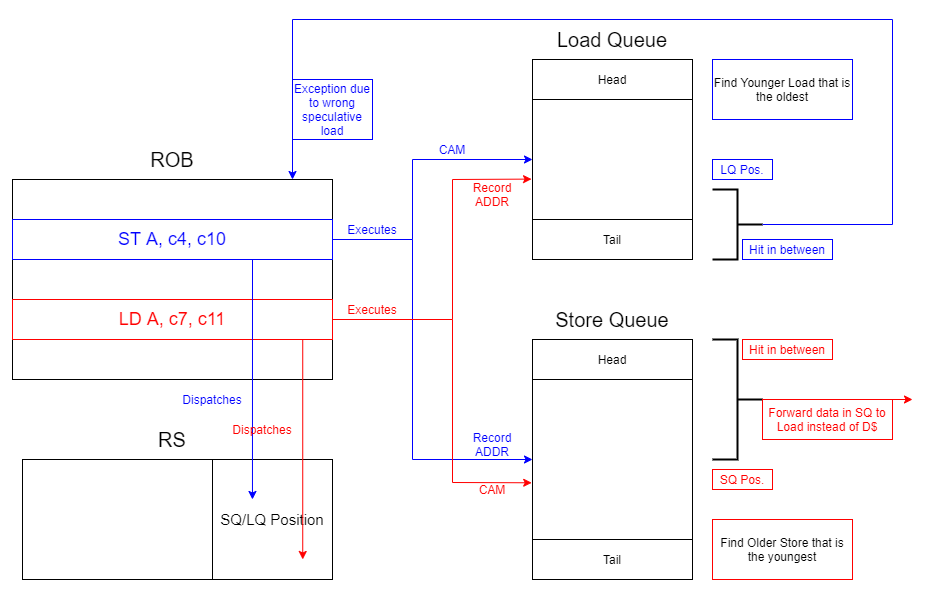
\includegraphics[width=.8\textwidth]{14.png}}
  \caption{Load and SQ}
\end{figure*}

\section{Branch Prediction}
\subsection*{Dynamic Branch Prediction}
A branch predictor consists of two parts: (1) target predictor (BTB) and (2) direction predictor (BHT/PHT). BTB supplies \textbf{branched target PC} and BHT/PHT predicts \textbf{whether to take a branch} or not.

\subsubsection*{BTB}
BTBs work because instruction targets are stable and indirect conditional branches are not widely supported. BTBs also support indirect calls like DLLs since stitched libraries may result in different targets on every execution, the target remains the same in a given run. Unconditional jumps can be further supported with Return Address Stack (RAS).

\subsubsection*{RAS}
Function calls are well-tracked using stacks. Push a \texttt{PC+4} into the RAS when seeing a \texttt{jump} and pop the entry when seeing a \texttt{return} instruction.

\begin{figure}[H]
    \centering
    {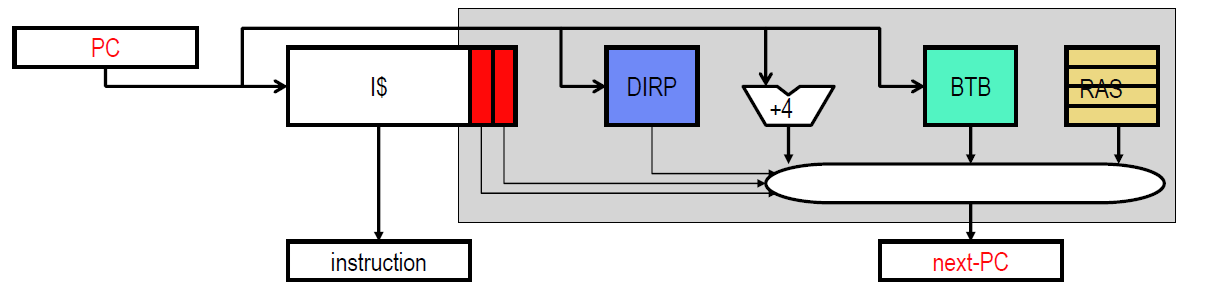
\includegraphics[width=.45\textwidth]{RAS.png}}
  \caption{Organization of RAS and BTB}
\end{figure}

\subsection*{Local Branch Prediction}
Individual (local) branches are often unbiased/weakly biased. 
\subsubsection*{One-level predictor}
Easiest way is to maintain a pattern history table (PHT) indexed by partial bits of branch PC to lookup direction prediction. For single direction predictor, change upon wrong prediction. For 2-bit saturating counters, direction transitions to state of branch result.
\subsubsection*{Two-level predictor}
Since branch outcomes can be correlated, a Branch History Table (BHT) records a window of outcomes for a branch and the window indexes a PHT.

\begin{figure}[H]
    \centering
    {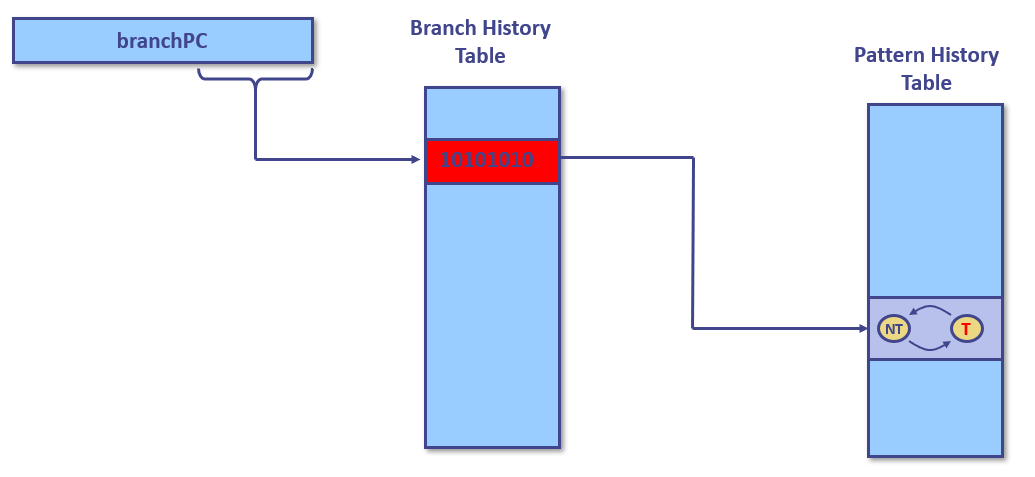
\includegraphics[width=.45\textwidth]{2level_pred.png}}
  \caption{Organization of 2-level Predictor}
\end{figure}

\begin{figure}[H]
    \centering
    {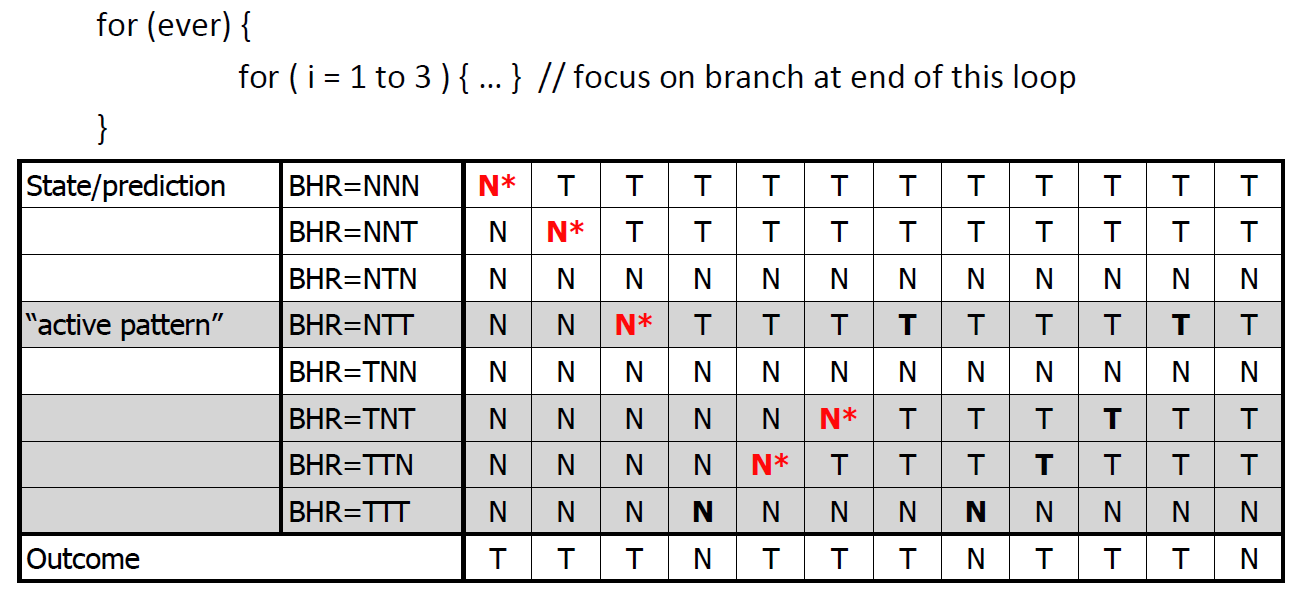
\includegraphics[width=.45\textwidth]{corr_pred.png}}
  \caption{Correlation Prediction Example}
\end{figure}

\subsection*{Global Branch Prediction}
Certain branches don't correlate with past iterations but instead all branches. Global predictor can learn correlation between outcome of different branches.
\subsubsection*{Simple Global Branch}
Use only one Branch History Register (BHR) to store outcome of all branches (in sequence) and use the register value to index into a pattern history table (PHT). Problem is that if two branches are \textbf{too close to each other}, the later branch will not see the latest outcome to make a prediction if the older branch has not retired.

\subsubsection*{GShare Global Branch}
Hash the global BHR with bits of the branch PC to index to the PHT. Hashes combines different inputs instead of concatenating them which would cause size explosions in lookup tables. PHT can be made bigger to avoid collisions.

\section{Instruction Prefetch}
\subsection*{Why Prefetch?}
Main motivation being speed difference between CPU and memory is getting larger.
\subsubsection*{Conventional approaches}
{[1]}: Avoid main memory access by adding cache hierarchy but has diminishing returns and is difficult for multi-core systems (coherence)
\medskip\hrule\medskip\noindent
{[2]}: Hide main memory latency by employing OoO but issue logic and LSQ is hard to scale up and it doesn't help dependent instructions.

\subsubsection*{Software Prefetching}
Compiler/ISA support prefetch instructions. Binding prefetches into registers (acts like \textbf{move loads early})

\subsubsection*{Hardware Prefetching}
Design choices include \textbf{what} (a block spatially head/address predictors) and \textbf{when} (on every miss/reference) to prefetch. A \textbf{large cache block} itself has the effect of prefetching as well.

\subsection*{Prefetchers}
\subsubsection*{Sequential Prefetcher (I\$)}
Can prefetch on cache misses: A FSM could throw new requests to memory while waiting for missed data to come back.
\par\noindent
Usually works well for I\$ but not D\$

\subsubsection*{Stride Prefetcher (D\$)}
Walking through a matrix/array might be \textbf{a consistent stride in memory}, so we can use the RPT to see if the prefetcher can exploit the loading pattern. When executing loads, look in RPT and see if new distance (current address - last address) matches old stride, prefetch (addr+stride) and update last address and last stride. Good for avoiding compulsory misses.

\begin{figure}[H]
    \centering
    {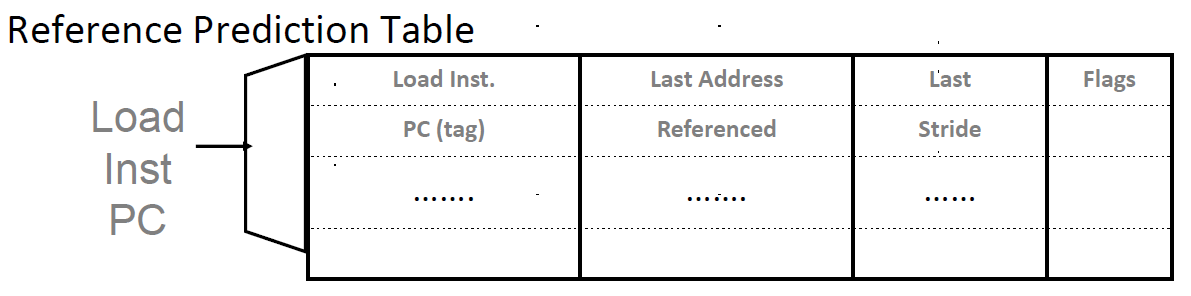
\includegraphics[width=.45\textwidth]{17.png}}
  \caption{Stride Prefetch}
\end{figure}

\subsubsection*{Stream Prefetcher (D\$)}
Use couple of auxiliary FIFO queues as space for prefetched data. When miss in D\$, look at head of all FIFO queues. If match, update cache with the data and pop entry from the FIFO queue; otherwise, allocate a new stream. The queues also have a LRU policy upon allocation of new streams when all queues are used. This prefetcher \textbf{avoids cache pollution}.

\begin{figure}[H]
    \centering
    {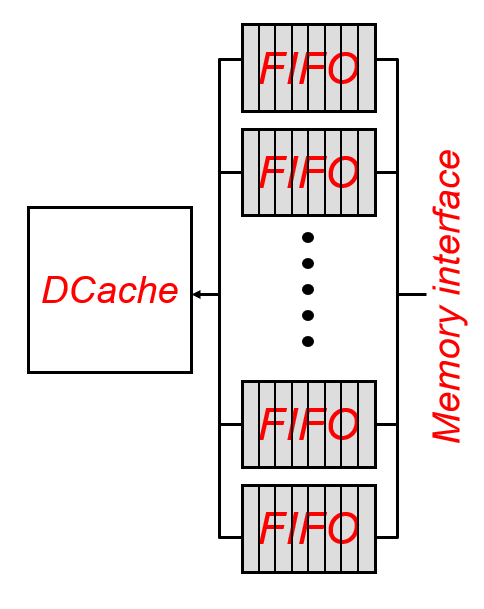
\includegraphics[width=.45\textwidth]{18.png}}
  \caption{Stream Prefetch}
\end{figure}

\subsubsection*{Runahead Prefetcher}
Duplicate the program and another thread only executes the address generating stream. Could be used to predict values for addresses/control flow. Predicts (1) control flow (branch), (2) address generation computation.

\subsubsection*{Coorelation-Based Prefetcher}
Track the likely next addresses after seeing a particular address via generated Markov model. Effective for prefetching linked lists.

\begin{figure}[H]
    \centering
    {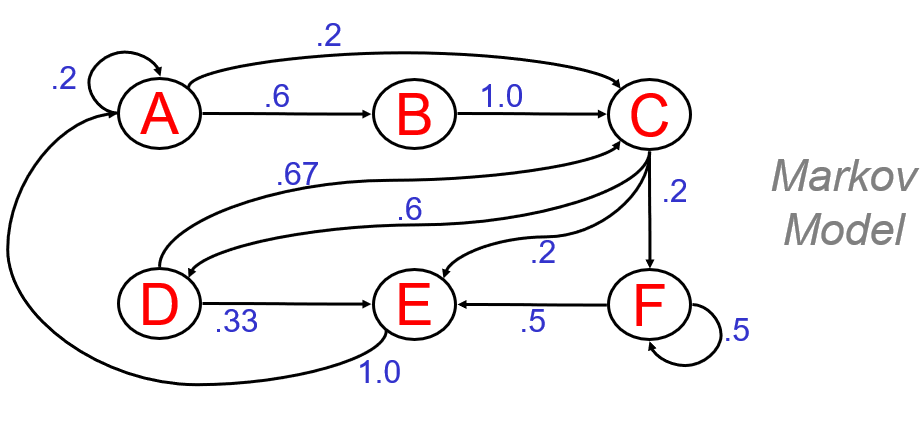
\includegraphics[width=.45\textwidth]{19.png}}
  \caption{Correlation Prefetch}
\end{figure}

\section{Virtual Memory}

\subsection*{Motivation}
\subsubsection*{Multiprogramming}
We want multiple running processes and each program might use the same address.

\subsubsection*{Demand Paging}
We can't scale up the address space: \\
32bit $\rightarrow$ 4GB; 48bit $\rightarrow$ 256TB \\
And what if storage of programs is larger than memory available physically?

\subsection*{Mechanism Evolution}
\subsubsection*{Base and Bound}
Each process sees a private and uniform address space. Main disadvantage is the requirement of regions being contiguous.

\begin{figure}[H]
    \centering
    {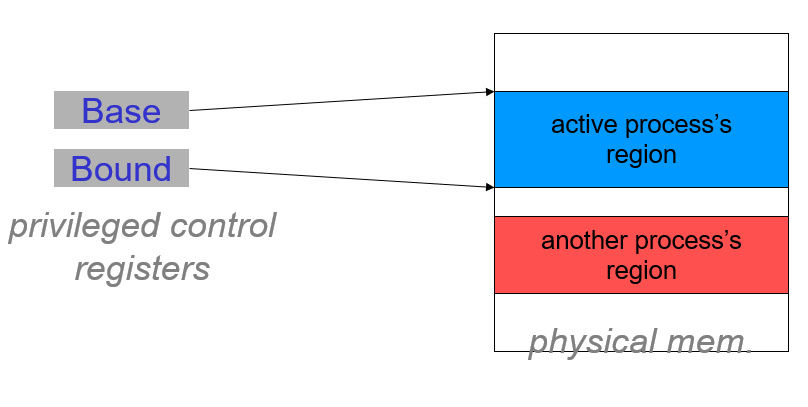
\includegraphics[width=.45\textwidth]{20.png}}
  \caption{Base and Bound}
\end{figure}

\subsubsection*{Segmented Address}
Each segment is a base and bound pair. Each process has multiple segments. The \textbf{segment table} is unique to each process.

\begin{figure}[H]
    \centering
    {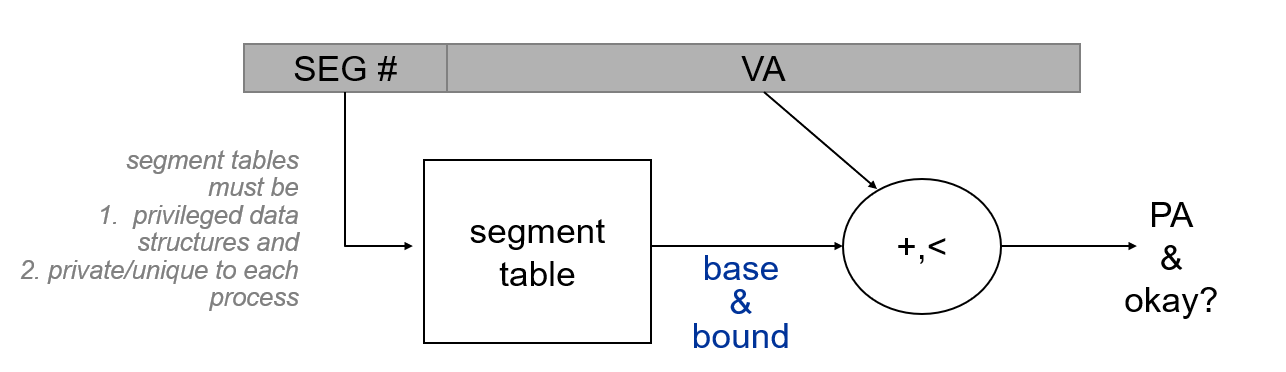
\includegraphics[width=.45\textwidth]{21.png}}
  \caption{Segment Address}
\end{figure}

\subsubsection*{Paged Address}
Segments are all of same size (4KB) and VA is interpreted as page number and page offset. The \textbf{page table} is unique to each process.

\begin{figure}[H]
    \centering
    {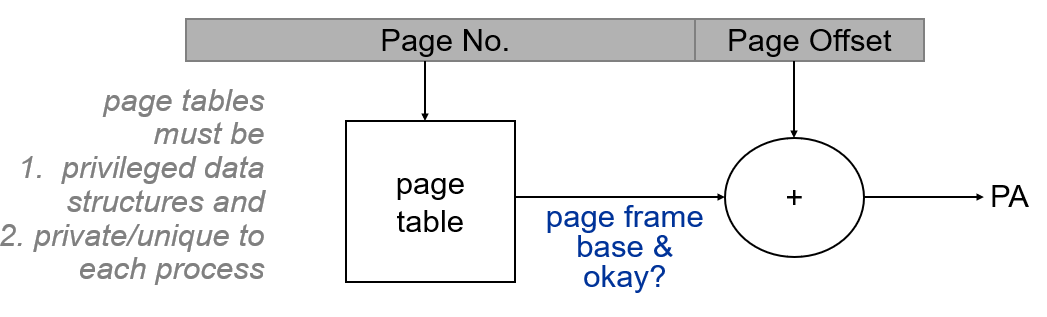
\includegraphics[width=.45\textwidth]{22.png}}
  \caption{Paged Address}
\end{figure}

\subsection*{Page Table Organization}
No need for a big table to contiguously list all physical page numbers. Could instead use \textbf{Hierarchical map} or \textbf{Inverted (hash)} page tables.

\begin{figure}[H]
    \centering
    {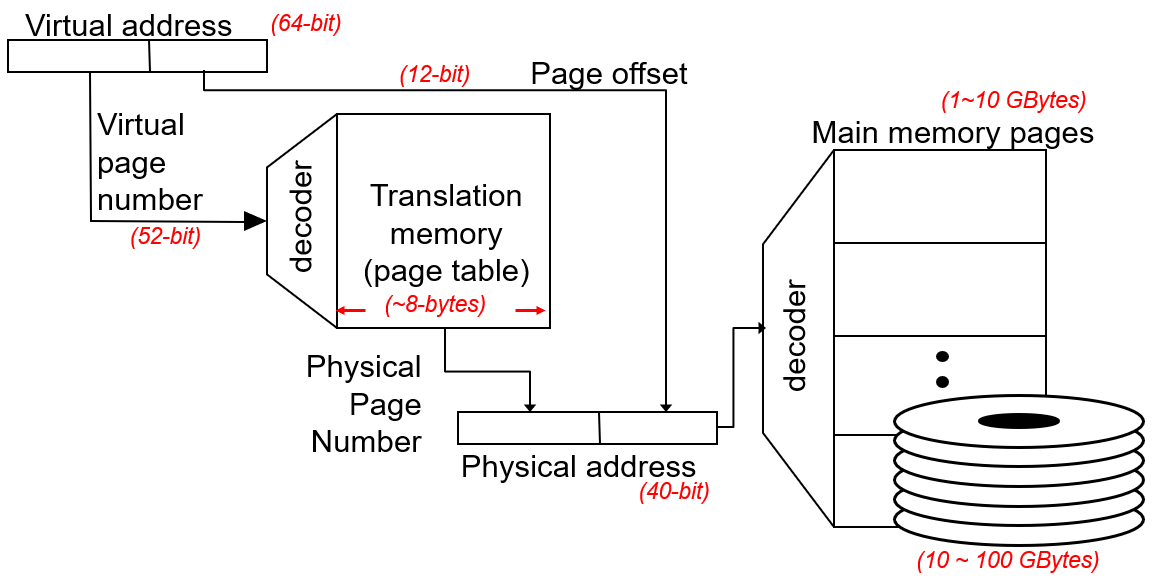
\includegraphics[width=.45\textwidth]{23.png}}
  \caption{Page Table Organization}
\end{figure}

\subsubsection*{Hierarchical Page Table}
Use different parts of the effective address to index to different hierarchy levels. Worst case would store the extra table of page tables (not expensive).

\begin{figure}[H]
    \centering
    {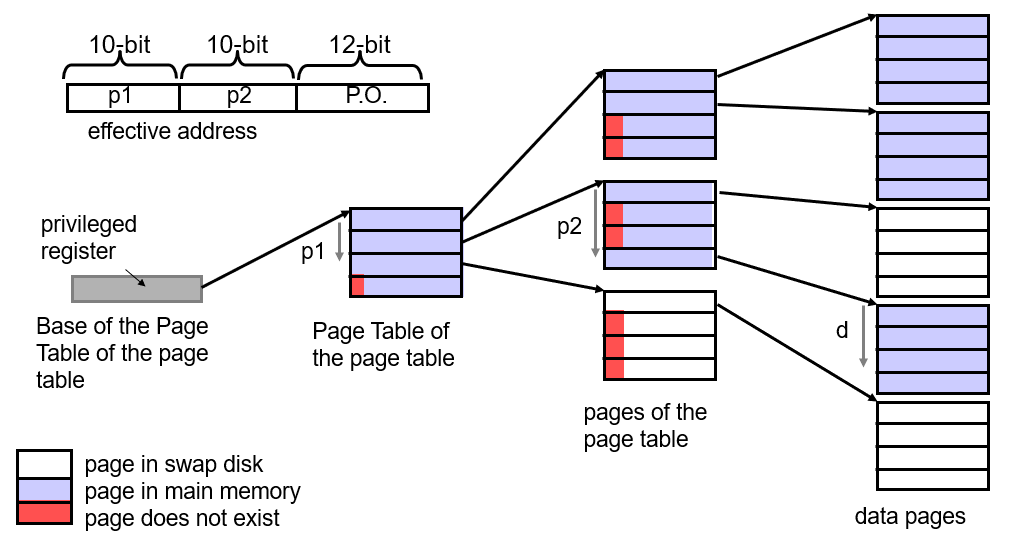
\includegraphics[width=.45\textwidth]{24.png}}
  \caption{Hierarchical Page Table}
\end{figure}

\subsubsection*{Hash Page Table}
Hash the Process ID and virtual page number before adding to the page table base address which acts as the index to the page table. Each entry of the table also stores a VPN/PID pair that would check for conflicting accesses. Less memory lookups compared to the hierarchical page table.

\begin{figure}[H]
    \centering
    {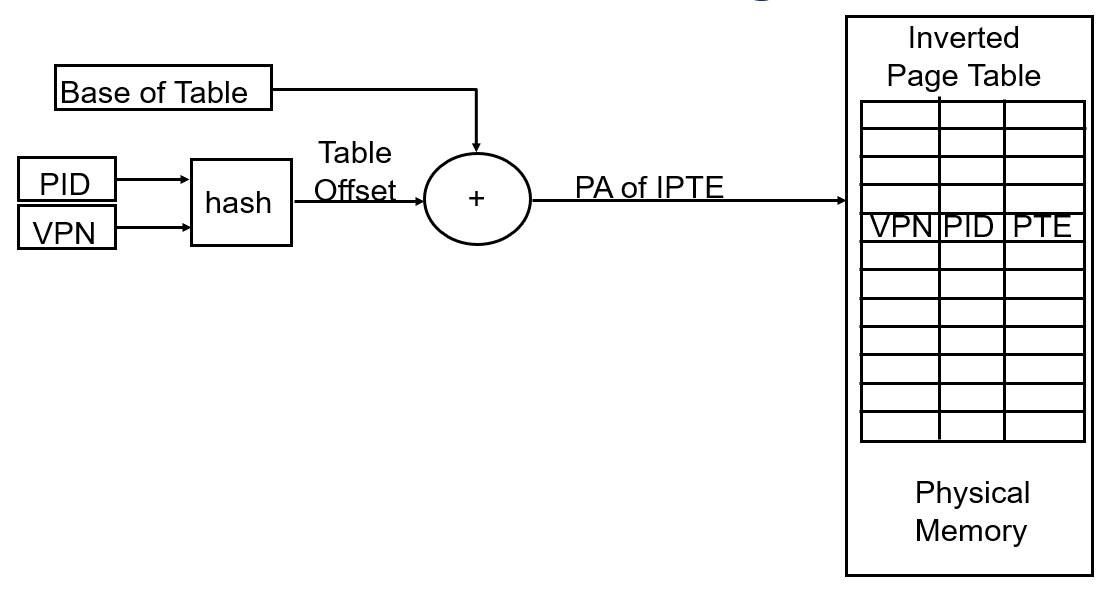
\includegraphics[width=.45\textwidth]{25.png}}
  \caption{Hash Page Table}
\end{figure}

\subsection*{Translation Look-aside Buffer}
Motivation is to avoid going to the page table on every reference. (Similar to caches)
\medskip\par\noindent
Uses lower bits of VPN to access the TLB and upper bits acts as tags which contains the PID for multi-process systems. Data of a TLB entry contains physical page number and access permissions.

\begin{figure}[H]
    \centering
    {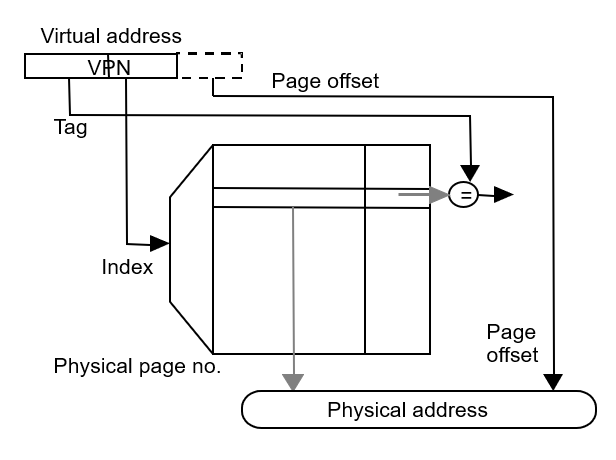
\includegraphics[width=.45\textwidth]{26.png}}
  \caption{TLB}
\end{figure}

\subsubsection*{TLB placement}
Where exactly does the address get translated? Before or after cache accesses? Physical caches have longer hit times due to translation latency. Virtual caches only translates on misses but address aliasing has to be handled by flushing the cache on each context switch.

\begin{figure}[H]
    \centering
    {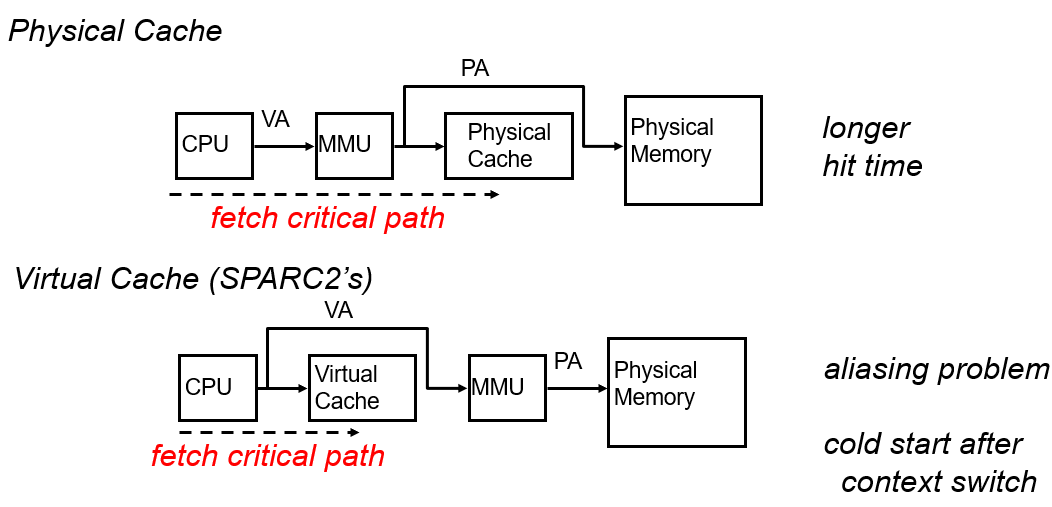
\includegraphics[width=.45\textwidth]{28.png}}
  \caption{TLB Placement Consideration}
\end{figure}

\begin{figure}[H]
    \centering
    {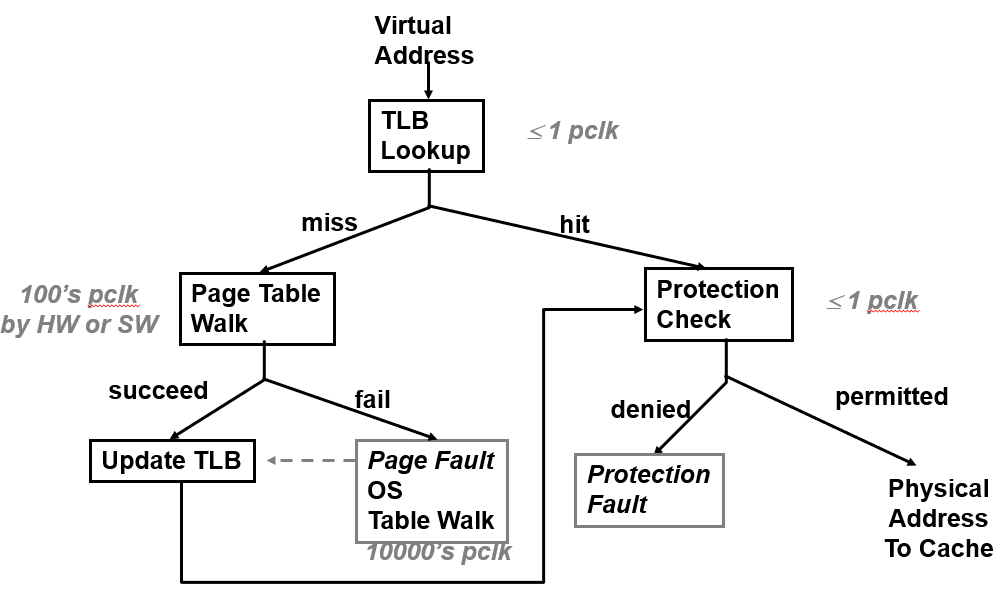
\includegraphics[width=.45\textwidth]{27.png}}
  \caption{Translation Procedure}
\end{figure}

\subsection*{Translation and Caches}
\subsubsection*{VIVT Caches}
Virtual index and tags allow cache accesses right away without translation at the cost of homonyms (1 virtual to many physical) and synonyms (many virtual to 1 physical). Read-only caches don't have to deal with synonyms while we could flush cache or include ASID tags to distinguish homonyms.
\medskip\par\noindent
Have to flush cache (must for synonym) after context switch or add PID to cache.

\begin{figure}[H]
    \centering
    {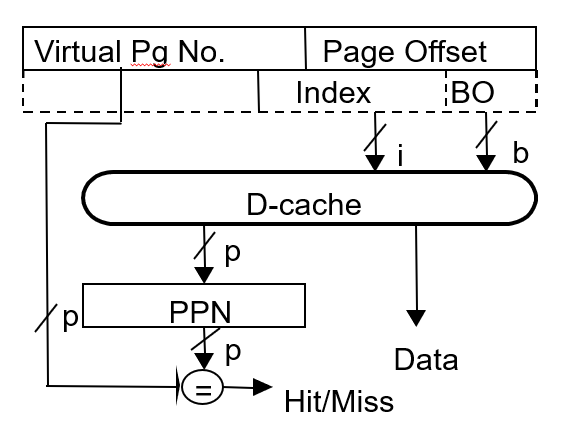
\includegraphics[width=.35\textwidth]{29.png}}
  \caption{VIVT Indexing}
\end{figure}

\subsubsection*{PIPT Caches}
No homonyms and synonyms but is slow due to translation.

\begin{figure}[H]
    \centering
    {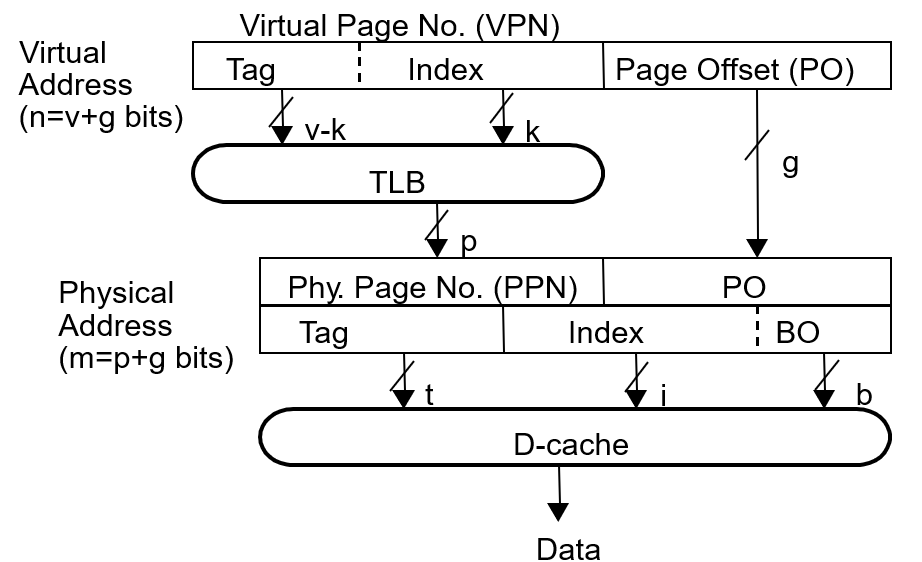
\includegraphics[width=.45\textwidth]{30.png}}
  \caption{PIPT Indexing}
\end{figure}

\subsubsection*{VIPT Caches}
If \textbf{data cache is small enough}, the higher bits of the page offset is enough to index into the data cache. Note that the page offset stays the same even after translation. 
\medskip\par\noindent
If index uses the translated regions (cache too large hence index uses too much bits), then 2 indices that are different in the exceeded bits might map to the same physical page.

\begin{figure}[H]
    \centering
    {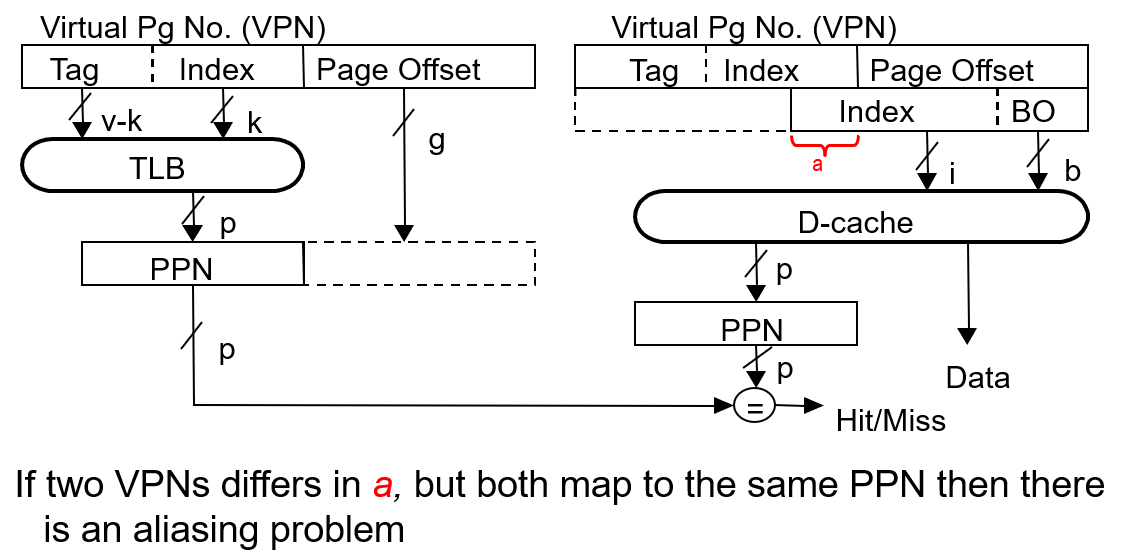
\includegraphics[width=.45\textwidth]{31.png}}
  \caption{VIPT Indexing}
\end{figure}

\section{Multiprocessors}
Thread level parallelism is a collection of asynchronous tasks: \textbf{not started and stopped together} and is coarser than instruction parallelism (thousands of instructions).
\subsection*{Shared Memory}
Easier for programmer to think about. Hardware is handling implicit communications, meaning synchronization is difficult.

\subsection*{Separate Processor/Memory?}
UMA has equal latency since \textbf{all} processor goes through a bus to reach memory banks. NUMA can access local memory with synchronization complexities.

\begin{figure}[H]
    \centering
    {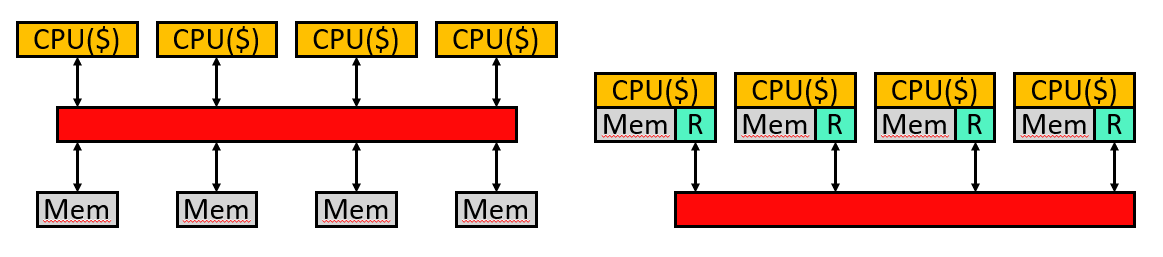
\includegraphics[width=.45\textwidth]{32.png}}
  \caption{UMA v.s. NUMA}
\end{figure}

\subsection*{Shared Network?}
A bus (shared network) has low latency but has low bandwidth (can't scale). A ring/mesh topology needs more hops to communicate but can scale up with more complex coherence protocols. Other network structures include trees.

\begin{figure}[H]
    \centering
    {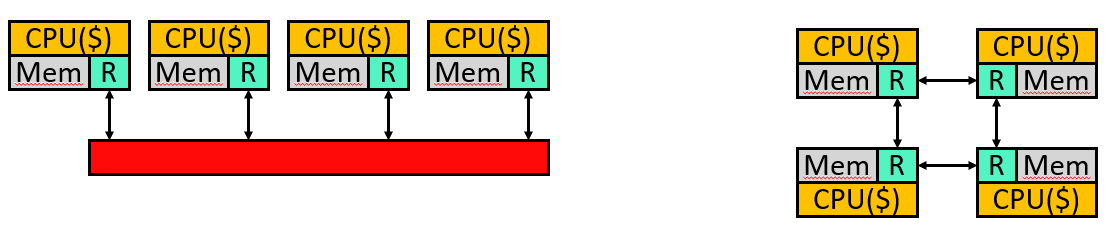
\includegraphics[width=.45\textwidth]{33.png}}
  \caption{Bus v.s. Scalable MP}
\end{figure}

\subsection*{Cache Coherence}
Thread-level parallelism issue (1): Multiple caches meant that they can get out-of-sync (incoherent).
\medskip\par\noindent
Fix with \textbf{coherence protocols}.
\subsubsection*{Protocol Design}
Define actions upon \textbf{events} (from either processor or bus) for each cache block. Each block maintains a particular state. Express transitions using \textbf{state machines}.

\subsubsection*{Simple write-through (Valid/Invalid)}
When storing, throw a write message onto the bus and all other caches snoop bus traffic. (\textbf{write-through + no-write-allocate caches}) (Insert Lec 19 Slide 21)
\medskip\par\noindent
Why not a good idea? Hogs ton of process to memory bandwidth (write-through) and most likely the cores would update the block again before the initial store is resolved in memory.

\begin{figure}[H]
    \centering
    {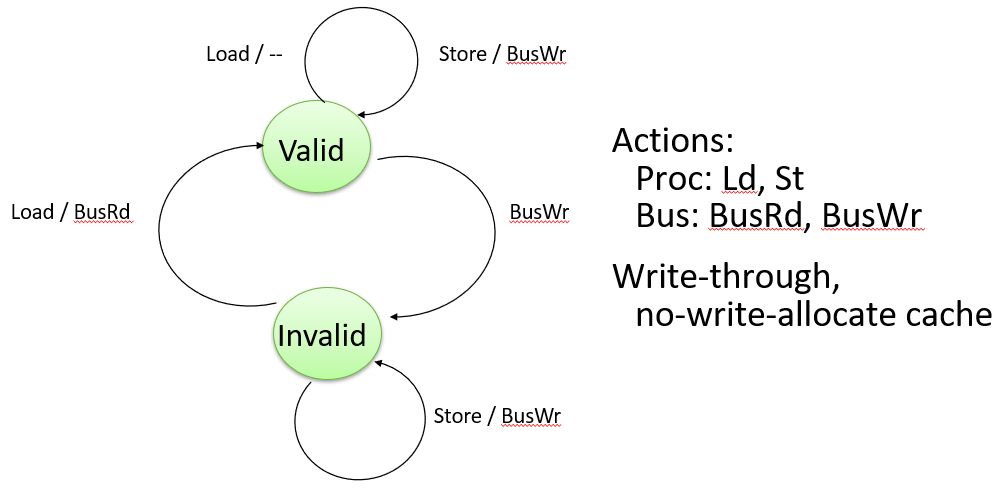
\includegraphics[width=.45\textwidth]{34.png}}
  \caption{I/V Protocol}
\end{figure}

\subsubsection*{Supporting Write-Back (MSI)}
Write-Back caches saves lots of bandwidth but needs notion of "ownership" -- \textbf{Mutual} exclusion (can update freely) and \textbf{Sharing} (allow multiple readers but not allowed to write).

\begin{figure}[H]
    \centering
    {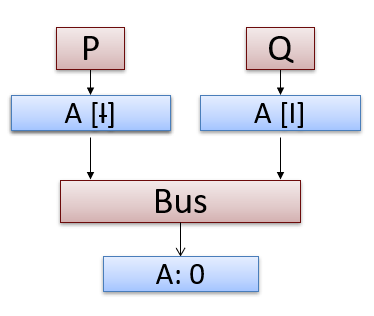
\includegraphics[width=.25\textwidth]{35.png}}
  \caption{Example Setup}
\end{figure}

\medskip\par\noindent
\smallskip\hrule\smallskip\noindent
[I$\rightarrow$S]: Initially \textbf{invalid} and if see load \textit{A} from processor \textbf{P} (miss), move to \textbf{shared} and issue \textbf{\texttt{BusRd}}.

\smallskip\hrule\smallskip\noindent
[S$\rightarrow$S]: (1)Processor \textbf{P} loads \textit{A} again and hit in cache. Since at \textbf{shared} means it's allowed to read from it. No need to issue bus messages to waste bandwidth.\\ 
(2) Processor \textbf{Q} also loads \textit{A} (cache miss), issues \textbf{\texttt{BusRd}} and then gets \textbf{\texttt{BusReply}}.

\smallskip\hrule\smallskip\noindent
[S$\rightarrow$I]: (1) Processor \textbf{Q} brought something into cache and kick \textit{A} out (eviction). No need to update \textit{A}, just directly move back to invalid without bus messages.\\
(2) Processor \textbf{Q} stores to \textit{A} and sends out \textbf{\texttt{BusRdX} \textit{A}}. Processor \textbf{P} with shared A replies (\textbf{\texttt{BusReply} \textit{A}}) then invalidates itself (Honoring exclusive access). Processor \textbf{Q} moves to \textbf{modified}.

\smallskip\hrule\smallskip\noindent
[M$\rightarrow$M]: While in \textbf{modified}, the block stays at \textbf{modified} if processor \textbf{Q} loads/stores to it.

\smallskip\hrule\smallskip\noindent
[M$\rightarrow$S]: Processor \textbf{P} has \textbf{invalid} block and issues \textbf{\texttt{BusRd}}, Processor \textbf{Q} with \textbf{modified} block replies with \textbf{\texttt{BusReply}} and demotes to \textbf{shared} state. \ctext[RGB]{232,209,82}{Main memory snarfs the value from Processor \textbf{Q} and updates its value.} (When downgrading, memory has to be updated!)

\smallskip\hrule\smallskip\noindent
[S/I$\rightarrow$M]: Processor \textbf{P} stores to \textit{A} (upgrade) and \textit{A} in Processor \textbf{Q} replies with \textbf{\texttt{BusReply}} then demotes to \textbf{invalid}.

\smallskip\hrule\smallskip\noindent
[M$\rightarrow$I]: (1) Processor \textbf{Q} sees \textbf{\texttt{BusRdx}} from Processor \textbf{P} and replies with \textbf{\texttt{BusReply}} then demotes to \textbf{invalid}\\
(2) Processor \textbf{Q} evicts \textit{A} from cache then issues \textbf{\texttt{BusWB}}.

\begin{figure}[H]
    \centering
    {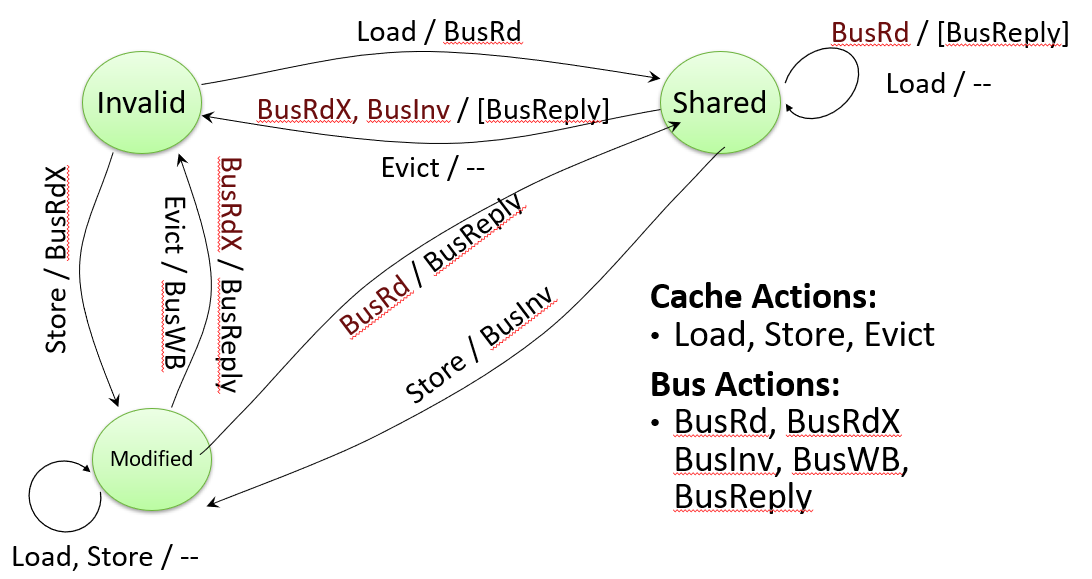
\includegraphics[width=.45\textwidth]{36.png}}
  \caption{MSI Protocol}
\end{figure}

\subsubsection*{Relaxing Restrictions (MESI)}
MSI is being overly cautious, add exclusive state to reduce bus transactions. Most of the time the things a given thread is reading is not shared anywhere else (exclusiveness). A store on E allows silent upgrades (No need to issue bus message).

\begin{table}[H]
\centering
\begin{tabular}{|l|l|c|l|l|}
\hline
\multicolumn{5}{|c|}{Processor Actions}                                                       \\ \hline\hline
\multicolumn{1}{|c|}{\multirow{3}{*}{I}} & \multirow{3}{*}{$\rightarrow$} & \multicolumn{3}{c|}{M} \\ \cline{3-5} 
\multicolumn{1}{|c|}{}                   &                                & \multicolumn{3}{c|}{E} \\ \cline{3-5} 
\multicolumn{1}{|c|}{}                   &                                & \multicolumn{3}{c|}{S} \\ \hline\hline
E                                        & $\rightarrow$                  & \multicolumn{3}{c|}{M} \\ \hline
S                                        & $\rightarrow$                  & \multicolumn{3}{c|}{M} \\ \hline\hline
S                                        & $\rightarrow$                  & \multicolumn{3}{c|}{S} \\ \hline
E                                        & $\rightarrow$                  & \multicolumn{3}{c|}{E} \\ \hline
M                                        & $\rightarrow$                  & \multicolumn{3}{c|}{M} \\ \hline
\end{tabular}
\end{table}

\begin{table}[H]
\centering
\begin{tabular}{|l|l|l|}
\hline
\multicolumn{3}{|l|}{Bus Messages}           \\ \hline\hline
M & \multirow{3}{*}{$\rightarrow$} & \multirow{3}{*}{I} \\ \cline{1-1}
E & $\rightarrow$                  &                    \\ \cline{1-1}
S & $\rightarrow$                  &                    \\ \hline\hline
M & $\rightarrow$                  & S                  \\ \hline
E & $\rightarrow$                  & S                  \\ \hline
\end{tabular}
\end{table}

\subsubsection*{Scalable Coherence}
Maintain a directory for ownership of cache blocks. Writer has to get confirmation of owner (listed in directory) before updating a cache block.
\medskip\par\noindent
\textbf{Single directory isn't scalable!} \textbf{Distributed} nodes (i.e., Processor, Cache, Memory, Directory) are connected via an interconnect (P2P/Ring, not a bus). Memory of different nodes map to different addresses (1st Node 0--1GB, 2nd Node 1--2GB, etc.)
\medskip\par\noindent
Each distributed directory maintains the status of each block (MESI and the processors that read the block). Since memory addresses are "distributed", the network interface of each processor knows where to send a request (point to point). [see youtube link]

\subsection*{Memory Consistency}
Thread-level parallelism issue (2): OoO makes it harder to ensure ordering of memory operations across threads.
\medskip\par\noindent
Define consistency model for specifying additional memory orderings.
\subsubsection*{Dekker's Algorithm:}
Dekker's Algorithm: Operating systems only allow one thread in critical region of code (e.g., only one update to a bank account)

\section{Multithreading}
Threads are logical sequence of instructions that share register values and address space.
\medskip\par\noindent
Multithreading run multiple threads that may or may not share an address space but each has their own register values.
\medskip\par\noindent
Multithreading trades latency for throughput (improves aggregated latency)

\subsection*{Core Sharing}
\subsubsection*{Time Sharing}
Switch to thread that has been waiting the longest when encountering long-latency operations. (Greedy than oldest)
\subsubsection*{Space Sharing}
Share across pipeline width and depth. Fetch and issue multiple threads each cycle. (SMT/Hyper-threading)

\subsection*{Execution Schemes}
\subsubsection*{Single Way}
Blanks can be dependencies/branch mispredicts. Colored blocks represent a valid instruction occupying a certain stage of the pipeline.

\subsubsection*{Superscalar}
Higher width implies better performance but also meant that more opportunities for more dependencies/mispredicts; hence lower utilization overall.

\subsubsection*{Predicate}
Execute all instructions regardless of the if condition. Throw away invalid results at writeback.

\subsubsection*{CMP}
Each thread has half (2-core) resources. Low core utilization if not much threads are present.

\subsubsection*{Coarse-Grain}
Switch to another thread when current thread encounters long latency instruction (e.g. L2 Miss). Preserves single thread performance. 
\medskip\par\noindent
Follows a thread scheduling policy by assigning a preferred thread to only switch away when long latencies occur and switch back when it's done. Computation resources are not shared at a given time.
\medskip\par\noindent
Flush pipeline on switch to prevent fake data dependencies (Different threads have independent register values). Short, in-order pipeline for good performance.
\medskip\par\noindent
When number of threads running is larger than virtual cores, OS writes out register file and thread state to memory to allocate space for another thread.

\subsubsection*{Fine-Grain}
Add complexity to allow multiple threads in the pipeline at a given time (round-robin scheduling). May take several cycles to rotate back to a given thread. $\rightarrow$ less stalls.
\medskip\par\noindent
Longer time to complete individual thread but allows higher utilization. Allows longer pipeline since no flushing. Needs larger register file for multiple threads.

\subsubsection*{Simultaneous}
Multi-threading on an OoO machine.
\medskip\par\noindent
Replicate Map-Table but share physical register file $\rightarrow$ Dynamically choose how much of register file is used for a thread. (Map Table: Dynamically allocate PR to different AR; Map Table w/ SMT: also to different threads)
\medskip\par\noindent
Only single thread workload $\rightarrow$ No need to partition PR and ROB, treat as single-threaded machine at no cost.

\subsection*{Multi-threading issues}
(1) \textbf{Cache interference} and (2) \textbf{resource contention}. Threads sharing memory can avoid contention (Suitable in servers). Resource partitioning can be static (equal-size, low utilization, no starvation) or dynamic (high utilization and possible starvation).

\end{multicols*}

\end{document}

